% Created by tikzDevice version 0.12.6 on 2026-05-04 16:15:57
% !TEX encoding = UTF-8 Unicode
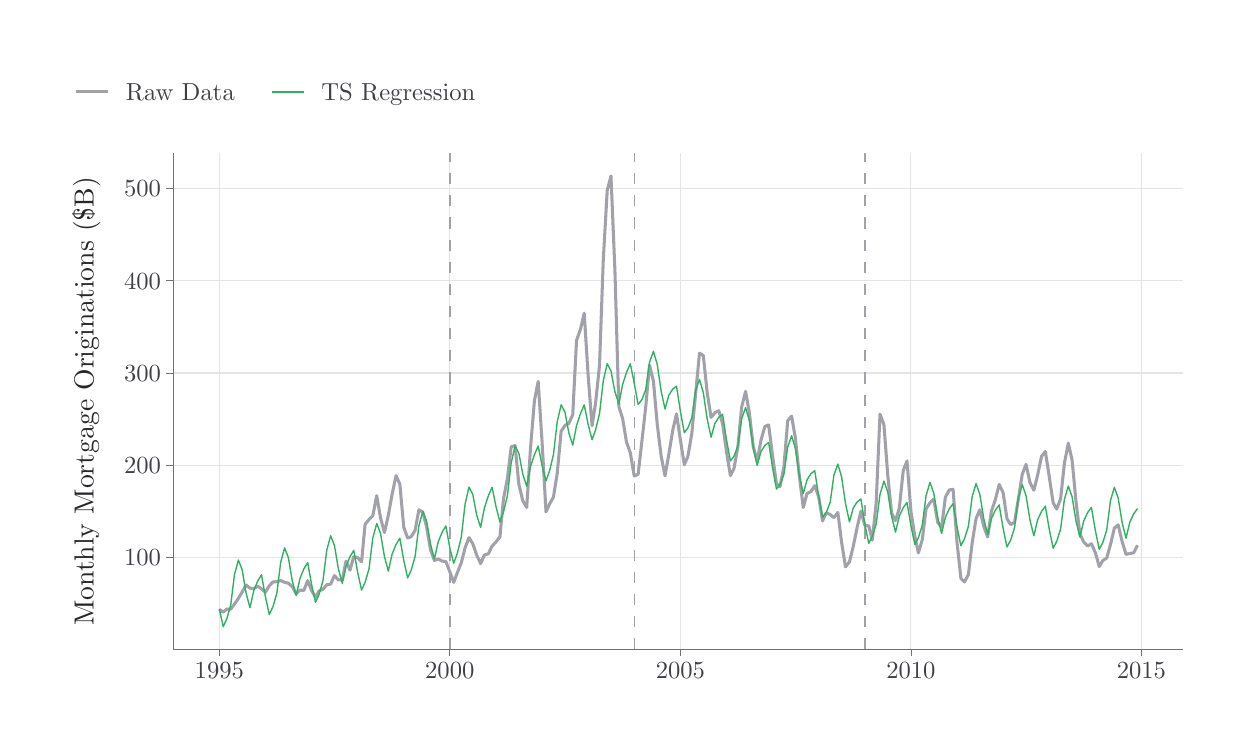
\begin{tikzpicture}[x=1pt,y=1pt]
\definecolor{fillColor}{RGB}{255,255,255}
\path[use as bounding box,fill=fillColor] (0,0) rectangle (433.62,252.94);
\begin{scope}
\path[clip] (  0.00,  0.00) rectangle (433.62,252.94);
\definecolor{drawColor}{RGB}{255,255,255}

\path[draw=drawColor,line width= 0.5pt,line join=round,line cap=round,fill=fillColor] ( -0.00,  0.00) rectangle (433.62,252.94);
\end{scope}
\begin{scope}
\path[clip] ( 52.66, 28.35) rectangle (417.62,207.49);
\definecolor{drawColor}{RGB}{255,255,255}
\definecolor{fillColor}{RGB}{255,255,255}

\path[draw=drawColor,line width= 0.5pt,line join=round,line cap=round,fill=fillColor] ( 52.66, 28.35) rectangle (417.62,207.49);
\definecolor{drawColor}{RGB}{228,228,231}

\path[draw=drawColor,line width= 0.4pt,line join=round] ( 52.66, 61.49) --
	(417.62, 61.49);

\path[draw=drawColor,line width= 0.4pt,line join=round] ( 52.66, 94.83) --
	(417.62, 94.83);

\path[draw=drawColor,line width= 0.4pt,line join=round] ( 52.66,128.17) --
	(417.62,128.17);

\path[draw=drawColor,line width= 0.4pt,line join=round] ( 52.66,161.51) --
	(417.62,161.51);

\path[draw=drawColor,line width= 0.4pt,line join=round] ( 52.66,194.85) --
	(417.62,194.85);

\path[draw=drawColor,line width= 0.4pt,line join=round] ( 69.25, 28.35) --
	( 69.25,207.49);

\path[draw=drawColor,line width= 0.4pt,line join=round] (152.54, 28.35) --
	(152.54,207.49);

\path[draw=drawColor,line width= 0.4pt,line join=round] (235.87, 28.35) --
	(235.87,207.49);

\path[draw=drawColor,line width= 0.4pt,line join=round] (319.16, 28.35) --
	(319.16,207.49);

\path[draw=drawColor,line width= 0.4pt,line join=round] (402.44, 28.35) --
	(402.44,207.49);
\definecolor{drawColor}{RGB}{161,161,170}

\path[draw=drawColor,line width= 0.5pt,dash pattern=on 4pt off 4pt ,line join=round] (152.54, 28.35) -- (152.54,207.49);

\path[draw=drawColor,line width= 0.5pt,dash pattern=on 4pt off 4pt ,line join=round] (219.18, 28.35) -- (219.18,207.49);

\path[draw=drawColor,line width= 0.5pt,dash pattern=on 4pt off 4pt ,line join=round] (302.51, 28.35) -- (302.51,207.49);

\path[draw=drawColor,line width= 1.1pt,line join=round] ( 69.25, 42.75) --
	( 70.66, 41.72) --
	( 71.94, 42.87) --
	( 73.36, 42.80) --
	( 74.72, 44.62) --
	( 76.14, 46.70) --
	( 77.51, 49.01) --
	( 78.92, 51.56) --
	( 80.33, 50.42) --
	( 81.70, 50.23) --
	( 83.12, 51.16) --
	( 84.48, 50.17) --
	( 85.90, 48.92) --
	( 87.31, 51.32) --
	( 88.64, 52.68) --
	( 90.05, 52.74) --
	( 91.42, 53.19) --
	( 92.83, 52.51) --
	( 94.20, 52.19) --
	( 95.61, 50.96) --
	( 97.03, 48.35) --
	( 98.40, 49.72) --
	( 99.81, 49.57) --
	(101.18, 53.15) --
	(102.59, 49.55) --
	(104.01, 47.09) --
	(105.28, 49.41) --
	(106.70, 49.99) --
	(108.07, 51.64) --
	(109.48, 51.87) --
	(110.85, 54.95) --
	(112.26, 53.39) --
	(113.68, 53.35) --
	(115.04, 60.23) --
	(116.46, 56.91) --
	(117.83, 61.81) --
	(119.24, 61.44) --
	(120.65, 59.93) --
	(121.93, 73.53) --
	(123.35, 75.22) --
	(124.71, 76.63) --
	(126.13, 83.80) --
	(127.50, 75.84) --
	(128.91, 70.49) --
	(130.32, 76.72) --
	(131.69, 84.34) --
	(133.11, 91.06) --
	(134.48, 88.01) --
	(135.89, 72.49) --
	(137.30, 68.50) --
	(138.58, 69.03) --
	(139.99, 71.23) --
	(141.36, 78.71) --
	(142.78, 77.89) --
	(144.15, 72.49) --
	(145.56, 64.35) --
	(146.97, 60.39) --
	(148.34, 60.97) --
	(149.76, 60.20) --
	(151.12, 60.00) --
	(152.54, 56.31) --
	(153.95, 52.49) --
	(155.27, 56.05) --
	(156.69, 59.58) --
	(158.06, 65.01) --
	(159.47, 68.66) --
	(160.84, 66.46) --
	(162.25, 62.36) --
	(163.67, 59.27) --
	(165.04, 62.40) --
	(166.45, 62.81) --
	(167.82, 65.61) --
	(169.23, 67.12) --
	(170.65, 68.96) --
	(171.92, 82.56) --
	(173.34, 89.97) --
	(174.71,101.48) --
	(176.12,101.94) --
	(177.49, 87.95) --
	(178.90, 82.00) --
	(180.32, 79.58) --
	(181.68,100.81) --
	(183.10,118.02) --
	(184.47,125.13) --
	(185.88,103.20) --
	(187.29, 77.96) --
	(188.57, 80.79) --
	(189.98, 83.32) --
	(191.35, 91.90) --
	(192.77,107.12) --
	(194.14,109.20) --
	(195.55,109.93) --
	(196.96,113.10) --
	(198.33,139.95) --
	(199.75,143.96) --
	(201.11,149.78) --
	(202.53,127.08) --
	(203.94,109.07) --
	(205.22,117.40) --
	(206.63,130.86) --
	(208.00,169.21) --
	(209.42,194.12) --
	(210.78,199.35) --
	(212.20,165.16) --
	(213.61,116.04) --
	(214.98,111.71) --
	(216.39,103.16) --
	(217.76, 99.29) --
	(219.18, 90.89) --
	(220.59, 91.58) --
	(221.91,103.17) --
	(223.33,115.90) --
	(224.70,131.00) --
	(226.11,125.29) --
	(227.48,109.74) --
	(228.89, 98.26) --
	(230.31, 90.99) --
	(231.67, 98.75) --
	(233.09,107.42) --
	(234.46,113.40) --
	(235.87,103.87) --
	(237.28, 94.99) --
	(238.56, 98.00) --
	(239.98,106.29) --
	(241.34,120.43) --
	(242.76,135.34) --
	(244.13,134.48) --
	(245.54,121.05) --
	(246.95,112.12) --
	(248.32,113.82) --
	(249.74,114.51) --
	(251.10,109.82) --
	(252.52, 99.68) --
	(253.93, 91.07) --
	(255.21, 93.59) --
	(256.62,101.40) --
	(257.99,115.88) --
	(259.41,121.50) --
	(260.77,113.79) --
	(262.19,101.55) --
	(263.60, 96.22) --
	(264.97,103.86) --
	(266.38,108.81) --
	(267.75,109.40) --
	(269.17, 98.22) --
	(270.58, 88.12) --
	(271.86, 87.11) --
	(273.27, 94.39) --
	(274.64,110.96) --
	(276.05,112.56) --
	(277.42,104.53) --
	(278.84, 90.98) --
	(280.25, 79.55) --
	(281.62, 84.61) --
	(283.03, 85.32) --
	(284.40, 87.44) --
	(285.82, 83.43) --
	(287.23, 74.67) --
	(288.55, 77.63) --
	(289.97, 77.03) --
	(291.33, 75.90) --
	(292.75, 77.76) --
	(294.12, 66.88) --
	(295.53, 58.10) --
	(296.94, 59.91) --
	(298.31, 65.48) --
	(299.73, 72.39) --
	(301.10, 78.25) --
	(302.51, 73.06) --
	(303.92, 72.89) --
	(305.20, 67.75) --
	(306.61, 81.26) --
	(307.98,113.29) --
	(309.40,109.52) --
	(310.77, 91.43) --
	(312.18, 77.49) --
	(313.59, 74.80) --
	(314.96, 79.27) --
	(316.38, 92.83) --
	(317.74, 96.39) --
	(319.16, 78.19) --
	(320.57, 69.24) --
	(321.85, 63.15) --
	(323.26, 67.95) --
	(324.63, 79.04) --
	(326.05, 81.27) --
	(327.41, 82.60) --
	(328.83, 74.20) --
	(330.24, 72.38) --
	(331.61, 83.31) --
	(333.02, 85.90) --
	(334.39, 86.13) --
	(335.81, 66.99) --
	(337.22, 53.94) --
	(338.50, 52.63) --
	(339.91, 55.27) --
	(341.28, 66.72) --
	(342.69, 75.56) --
	(344.06, 78.71) --
	(345.48, 72.70) --
	(346.89, 68.88) --
	(348.26, 78.30) --
	(349.67, 82.36) --
	(351.04, 87.89) --
	(352.45, 85.00) --
	(353.87, 75.50) --
	(355.19, 73.39) --
	(356.61, 74.25) --
	(357.97, 82.61) --
	(359.39, 91.55) --
	(360.76, 95.16) --
	(362.17, 88.60) --
	(363.58, 85.80) --
	(364.95, 91.30) --
	(366.37, 98.05) --
	(367.73, 99.80) --
	(369.15, 90.66) --
	(370.56, 81.25) --
	(371.84, 78.99) --
	(373.25, 82.72) --
	(374.62, 95.57) --
	(376.04,102.79) --
	(377.40, 96.65) --
	(378.82, 81.59) --
	(380.23, 69.95) --
	(381.60, 67.12) --
	(383.01, 65.64) --
	(384.38, 66.45) --
	(385.80, 63.23) --
	(387.21, 58.23) --
	(388.49, 60.36) --
	(389.90, 61.29) --
	(391.27, 66.18) --
	(392.68, 72.09) --
	(394.05, 73.27) --
	(395.47, 67.30) --
	(396.88, 62.63) --
	(398.25, 62.91) --
	(399.66, 63.20) --
	(401.03, 65.91);
\definecolor{drawColor}{RGB}{45,178,95}

\path[draw=drawColor,line width= 0.5pt,line join=round] ( 69.25, 42.91) --
	( 70.66, 36.49) --
	( 71.94, 39.30) --
	( 73.36, 44.23) --
	( 74.72, 55.30) --
	( 76.14, 60.55) --
	( 77.51, 57.04) --
	( 78.92, 48.66) --
	( 80.33, 43.34) --
	( 81.70, 49.52) --
	( 83.12, 52.98) --
	( 84.48, 55.25) --
	( 85.90, 47.32) --
	( 87.31, 40.89) --
	( 88.64, 43.72) --
	( 90.05, 48.64) --
	( 91.42, 59.71) --
	( 92.83, 64.96) --
	( 94.20, 61.45) --
	( 95.61, 53.07) --
	( 97.03, 47.75) --
	( 98.40, 53.93) --
	( 99.81, 57.39) --
	(101.18, 59.67) --
	(102.59, 51.73) --
	(104.01, 45.31) --
	(105.28, 48.12) --
	(106.70, 53.04) --
	(108.07, 64.11) --
	(109.48, 69.36) --
	(110.85, 65.85) --
	(112.26, 57.47) --
	(113.68, 52.15) --
	(115.04, 58.33) --
	(116.46, 61.79) --
	(117.83, 64.07) --
	(119.24, 56.13) --
	(120.65, 49.71) --
	(121.93, 52.52) --
	(123.35, 57.44) --
	(124.71, 68.52) --
	(126.13, 73.76) --
	(127.50, 70.25) --
	(128.91, 61.88) --
	(130.32, 56.55) --
	(131.69, 62.73) --
	(133.11, 66.20) --
	(134.48, 68.47) --
	(135.89, 60.53) --
	(137.30, 54.11) --
	(138.58, 56.92) --
	(139.99, 61.84) --
	(141.36, 72.92) --
	(142.78, 78.16) --
	(144.15, 74.65) --
	(145.56, 66.28) --
	(146.97, 60.95) --
	(148.34, 67.13) --
	(149.76, 70.60) --
	(151.12, 72.87) --
	(152.54, 64.93) --
	(153.95, 59.40) --
	(155.27, 63.05) --
	(156.69, 68.87) --
	(158.06, 80.80) --
	(159.47, 86.94) --
	(160.84, 84.29) --
	(162.25, 76.80) --
	(163.67, 72.36) --
	(165.04, 79.40) --
	(166.45, 83.76) --
	(167.82, 86.89) --
	(169.23, 79.84) --
	(170.65, 74.31) --
	(171.92, 77.92) --
	(173.34, 83.73) --
	(174.71, 95.66) --
	(176.12,101.80) --
	(177.49, 99.15) --
	(178.90, 91.66) --
	(180.32, 87.23) --
	(181.68, 94.27) --
	(183.10, 98.62) --
	(184.47,101.75) --
	(185.88, 94.71) --
	(187.29, 89.17) --
	(188.57, 92.78) --
	(189.98, 98.60) --
	(191.35,110.53) --
	(192.77,116.67) --
	(194.14,114.02) --
	(195.55,106.53) --
	(196.96,102.09) --
	(198.33,109.13) --
	(199.75,113.49) --
	(201.11,116.62) --
	(202.53,109.57) --
	(203.94,104.04) --
	(205.22,107.65) --
	(206.63,113.46) --
	(208.00,125.40) --
	(209.42,131.53) --
	(210.78,128.88) --
	(212.20,121.39) --
	(213.61,116.96) --
	(214.98,124.00) --
	(216.39,128.35) --
	(217.76,131.49) --
	(219.18,124.44) --
	(220.59,116.78) --
	(221.91,118.44) --
	(223.33,122.12) --
	(224.70,132.00) --
	(226.11,136.01) --
	(227.48,131.30) --
	(228.89,121.68) --
	(230.31,115.12) --
	(231.67,120.10) --
	(233.09,122.33) --
	(234.46,123.40) --
	(235.87,114.23) --
	(237.28,106.57) --
	(238.56,108.26) --
	(239.98,111.94) --
	(241.34,121.82) --
	(242.76,125.82) --
	(244.13,121.11) --
	(245.54,111.50) --
	(246.95,104.94) --
	(248.32,109.92) --
	(249.74,112.14) --
	(251.10,113.22) --
	(252.52,104.04) --
	(253.93, 96.38) --
	(255.21, 98.07) --
	(256.62,101.76) --
	(257.99,111.63) --
	(259.41,115.64) --
	(260.77,110.93) --
	(262.19,101.32) --
	(263.60, 94.75) --
	(264.97, 99.73) --
	(266.38,101.96) --
	(267.75,103.04) --
	(269.17, 93.86) --
	(270.58, 86.20) --
	(271.86, 87.89) --
	(273.27, 91.57) --
	(274.64,101.45) --
	(276.05,105.46) --
	(277.42,100.75) --
	(278.84, 91.13) --
	(280.25, 84.57) --
	(281.62, 89.55) --
	(283.03, 91.78) --
	(284.40, 92.85) --
	(285.82, 83.68) --
	(287.23, 76.02) --
	(288.55, 77.68) --
	(289.97, 81.36) --
	(291.33, 91.24) --
	(292.75, 95.25) --
	(294.12, 90.54) --
	(295.53, 80.92) --
	(296.94, 74.36) --
	(298.31, 79.34) --
	(299.73, 81.57) --
	(301.10, 82.64) --
	(302.51, 73.47) --
	(303.92, 66.63) --
	(305.20, 69.07) --
	(306.61, 73.58) --
	(307.98, 84.26) --
	(309.40, 89.09) --
	(310.77, 85.18) --
	(312.18, 76.40) --
	(313.59, 70.66) --
	(314.96, 76.44) --
	(316.38, 79.50) --
	(317.74, 81.37) --
	(319.16, 73.02) --
	(320.57, 66.19) --
	(321.85, 68.63) --
	(323.26, 73.14) --
	(324.63, 83.82) --
	(326.05, 88.65) --
	(327.41, 84.74) --
	(328.83, 75.95) --
	(330.24, 70.22) --
	(331.61, 76.00) --
	(333.02, 79.05) --
	(334.39, 80.93) --
	(335.81, 72.58) --
	(337.22, 65.75) --
	(338.50, 68.18) --
	(339.91, 72.70) --
	(341.28, 83.37) --
	(342.69, 88.21) --
	(344.06, 84.30) --
	(345.48, 75.51) --
	(346.89, 69.78) --
	(348.26, 75.56) --
	(349.67, 78.61) --
	(351.04, 80.49) --
	(352.45, 72.14) --
	(353.87, 65.31) --
	(355.19, 67.74) --
	(356.61, 72.25) --
	(357.97, 82.93) --
	(359.39, 87.77) --
	(360.76, 83.86) --
	(362.17, 75.07) --
	(363.58, 69.33) --
	(364.95, 75.11) --
	(366.37, 78.17) --
	(367.73, 80.04) --
	(369.15, 71.69) --
	(370.56, 64.86) --
	(371.84, 67.30) --
	(373.25, 71.81) --
	(374.62, 82.49) --
	(376.04, 87.32) --
	(377.40, 83.41) --
	(378.82, 74.62) --
	(380.23, 68.89) --
	(381.60, 74.67) --
	(383.01, 77.73) --
	(384.38, 79.60) --
	(385.80, 71.25) --
	(387.21, 64.42) --
	(388.49, 66.86) --
	(389.90, 71.37) --
	(391.27, 82.04) --
	(392.68, 86.88) --
	(394.05, 82.97) --
	(395.47, 74.18) --
	(396.88, 68.45) --
	(398.25, 74.23) --
	(399.66, 77.28) --
	(401.03, 79.16);
\end{scope}
\begin{scope}
\path[clip] (  0.00,  0.00) rectangle (433.62,252.94);
\definecolor{drawColor}{RGB}{113,113,122}

\path[draw=drawColor,line width= 0.3pt,line join=round] ( 52.66, 28.35) --
	( 52.66,207.49);
\end{scope}
\begin{scope}
\path[clip] (  0.00,  0.00) rectangle (433.62,252.94);
\definecolor{drawColor}{RGB}{63,63,70}

\node[text=drawColor,anchor=base east,inner sep=0pt, outer sep=0pt, scale=  0.89] at ( 48.16, 58.43) {100};

\node[text=drawColor,anchor=base east,inner sep=0pt, outer sep=0pt, scale=  0.89] at ( 48.16, 91.77) {200};

\node[text=drawColor,anchor=base east,inner sep=0pt, outer sep=0pt, scale=  0.89] at ( 48.16,125.11) {300};

\node[text=drawColor,anchor=base east,inner sep=0pt, outer sep=0pt, scale=  0.89] at ( 48.16,158.45) {400};

\node[text=drawColor,anchor=base east,inner sep=0pt, outer sep=0pt, scale=  0.89] at ( 48.16,191.79) {500};
\end{scope}
\begin{scope}
\path[clip] (  0.00,  0.00) rectangle (433.62,252.94);
\definecolor{drawColor}{RGB}{113,113,122}

\path[draw=drawColor,line width= 0.3pt,line join=round] ( 50.16, 61.49) --
	( 52.66, 61.49);

\path[draw=drawColor,line width= 0.3pt,line join=round] ( 50.16, 94.83) --
	( 52.66, 94.83);

\path[draw=drawColor,line width= 0.3pt,line join=round] ( 50.16,128.17) --
	( 52.66,128.17);

\path[draw=drawColor,line width= 0.3pt,line join=round] ( 50.16,161.51) --
	( 52.66,161.51);

\path[draw=drawColor,line width= 0.3pt,line join=round] ( 50.16,194.85) --
	( 52.66,194.85);
\end{scope}
\begin{scope}
\path[clip] (  0.00,  0.00) rectangle (433.62,252.94);
\definecolor{drawColor}{RGB}{113,113,122}

\path[draw=drawColor,line width= 0.3pt,line join=round] ( 52.66, 28.35) --
	(417.62, 28.35);
\end{scope}
\begin{scope}
\path[clip] (  0.00,  0.00) rectangle (433.62,252.94);
\definecolor{drawColor}{RGB}{113,113,122}

\path[draw=drawColor,line width= 0.3pt,line join=round] ( 69.25, 25.85) --
	( 69.25, 28.35);

\path[draw=drawColor,line width= 0.3pt,line join=round] (152.54, 25.85) --
	(152.54, 28.35);

\path[draw=drawColor,line width= 0.3pt,line join=round] (235.87, 25.85) --
	(235.87, 28.35);

\path[draw=drawColor,line width= 0.3pt,line join=round] (319.16, 25.85) --
	(319.16, 28.35);

\path[draw=drawColor,line width= 0.3pt,line join=round] (402.44, 25.85) --
	(402.44, 28.35);
\end{scope}
\begin{scope}
\path[clip] (  0.00,  0.00) rectangle (433.62,252.94);
\definecolor{drawColor}{RGB}{63,63,70}

\node[text=drawColor,anchor=base,inner sep=0pt, outer sep=0pt, scale=  0.89] at ( 69.25, 17.73) {1995};

\node[text=drawColor,anchor=base,inner sep=0pt, outer sep=0pt, scale=  0.89] at (152.54, 17.73) {2000};

\node[text=drawColor,anchor=base,inner sep=0pt, outer sep=0pt, scale=  0.89] at (235.87, 17.73) {2005};

\node[text=drawColor,anchor=base,inner sep=0pt, outer sep=0pt, scale=  0.89] at (319.16, 17.73) {2010};

\node[text=drawColor,anchor=base,inner sep=0pt, outer sep=0pt, scale=  0.89] at (402.44, 17.73) {2015};
\end{scope}
\begin{scope}
\path[clip] (  0.00,  0.00) rectangle (433.62,252.94);
\definecolor{drawColor}{RGB}{39,39,42}

\node[text=drawColor,rotate= 90.00,anchor=base,inner sep=0pt, outer sep=0pt, scale=  1.00] at ( 23.86,117.92) {Monthly Mortgage Originations (\$B)};
\end{scope}
\begin{scope}
\path[clip] (  0.00,  0.00) rectangle (433.62,252.94);
\definecolor{drawColor}{RGB}{255,255,255}
\definecolor{fillColor}{RGB}{255,255,255}

\path[draw=drawColor,line width= 0.5pt,line join=round,line cap=round,fill=fillColor] ( 16.00,217.49) rectangle (161.70,236.95);
\end{scope}
\begin{scope}
\path[clip] (  0.00,  0.00) rectangle (433.62,252.94);
\definecolor{drawColor}{RGB}{255,255,255}
\definecolor{fillColor}{RGB}{255,255,255}

\path[draw=drawColor,line width= 0.5pt,line join=round,line cap=round,fill=fillColor] ( 16.00,222.49) rectangle ( 30.45,236.95);
\definecolor{drawColor}{RGB}{161,161,170}

\path[draw=drawColor,line width= 1.1pt,line join=round] ( 17.45,229.72) -- ( 29.01,229.72);
\end{scope}
\begin{scope}
\path[clip] (  0.00,  0.00) rectangle (433.62,252.94);
\definecolor{drawColor}{RGB}{255,255,255}
\definecolor{fillColor}{RGB}{255,255,255}

\path[draw=drawColor,line width= 0.5pt,line join=round,line cap=round,fill=fillColor] ( 86.70,222.49) rectangle (101.16,236.95);
\definecolor{drawColor}{RGB}{45,178,95}

\path[draw=drawColor,line width= 0.5pt,line join=round] ( 88.15,229.72) -- ( 99.71,229.72);
\end{scope}
\begin{scope}
\path[clip] (  0.00,  0.00) rectangle (433.62,252.94);
\definecolor{drawColor}{RGB}{63,63,70}

\node[text=drawColor,anchor=base west,inner sep=0pt, outer sep=0pt, scale=  0.89] at ( 35.45,226.66) {Raw Data};
\end{scope}
\begin{scope}
\path[clip] (  0.00,  0.00) rectangle (433.62,252.94);
\definecolor{drawColor}{RGB}{63,63,70}

\node[text=drawColor,anchor=base west,inner sep=0pt, outer sep=0pt, scale=  0.89] at (106.16,226.66) {TS Regression};
\end{scope}
\end{tikzpicture}
